% Metaphor: layered stack. Each layer rests on the one below and talks
% only to its neighbours -- reach for it when the reader's question is
% "what is allowed to depend on what".
%
% Idiom: stacked `fit` layers. A layer is a node drawn *around* its
% members rather than a rectangle at coordinates that happen to enclose
% them, so re-wording a member widens its layer instead of overflowing
% it. `review figure` treats containment as grouping rather than
% collision, which is exactly what this idiom is.
\usetikzlibrary{fit,positioning}
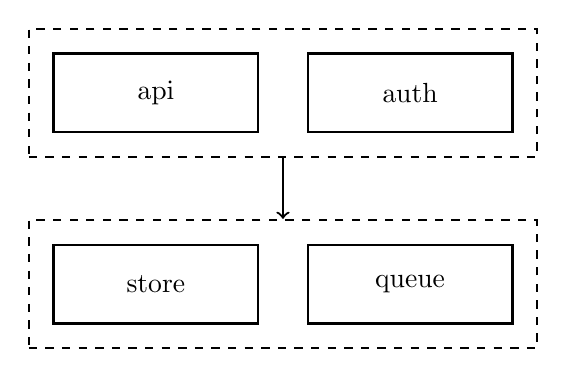
\begin{tikzpicture}[thick,
                    part/.style={draw,align=center,
                                 minimum width=26mm,minimum height=10mm},
                    layer/.style={draw,dashed,inner sep=3mm}]
  \node[part] (store) {store};
  \node[part,right=6mm of store] (queue) {queue};
  \node[layer,fit=(store)(queue)] (persistence) {};
  % 14mm between the *parts*, which is 8mm between the layers once each
  % `fit` box has taken its 3mm inner sep. Set this from the gap you
  % want between the layers, not between the parts: at 9mm here the
  % arrow between them had 3mm to live in and read as a smudge.
  \node[part,above=14mm of store] (api) {api};
  \node[part,right=6mm of api] (auth) {auth};
  \node[layer,fit=(api)(auth)] (service) {};
  \draw[->] (service) -- (persistence);
\end{tikzpicture}
